%% informe.tex -- Informe final CS5055 (P2), basado en acmmanuscript.tex (ACM Generic
%% Journal Manuscript). El original acmmanuscript.tex no se modifica.
%% nonacm: sin bloque de copyright, sin "ACM Reference Format", sin pie "Manuscript submitted".
%% natbib=false: las citas las resuelve IEEEtran.bst con \cite estándar ([1], [2], ...).
\documentclass[manuscript,screen,nonacm,natbib=false]{acmart}

\usepackage[spanish,es-noshorthands,es-tabla,es-nodecimaldot]{babel}
\usepackage{cite}
\usepackage{tabularx}
\usepackage{multirow}
\usepackage{xcolor}
\usepackage{amsmath}
\usepackage{placeins} % [section] choca con acmart; \FloatBarrier manual antes de cada \section
\usepackage{flafter}

\setcopyright{none}
\settopmatter{printacmref=false, printccs=false, printfolios=true}
\renewcommand\footnotetextcopyrightpermission[1]{}
\addto\captionsspanish{\renewcommand\keywordsname{Palabras clave}}
\authorsaddresses{}

%% Huecos que solo el equipo puede llenar (ver informe/PENDIENTES.md).
\newcommand{\pendiente}[1]{\textcolor{red}{[PENDIENTE: #1]}}
\newcommand{\gradC}{\textdegree{}C}
\newcommand{\COdos}{CO\textsubscript{2}}
\newcommand{\IIC}{I\textsuperscript{2}C}
\newcolumntype{Y}{>{\raggedright\arraybackslash}X}
\newcolumntype{P}[1]{>{\raggedright\arraybackslash}p{#1}}

\begin{document}

\title{Calienfriito: nodo IoT de control térmico y calidad de aire para aulas universitarias, con heurística activa y modelo de aprendizaje automático en modo sombra}
\renewcommand{\shorttitle}{Calienfriito: nodo IoT de control térmico y calidad de aire}

\author{Brayan Eduardo Gomero Castillo}
\affiliation{%
  \institution{Universidad de Ingeniería y Tecnología (UTEC)}
  \city{Lima}
  \country{Perú}}

\author{Kiara Alexandra Balcázar Santa Cruz}
\affiliation{%
  \institution{Universidad de Ingeniería y Tecnología (UTEC)}
  \city{Lima}
  \country{Perú}}

\author{Rodrigo Dion Carlos Acosta}
\affiliation{%
  \institution{Universidad de Ingeniería y Tecnología (UTEC)}
  \city{Lima}
  \country{Perú}}

\renewcommand{\shortauthors}{Gomero, Balcázar y Carlos}

\begin{abstract}
Las aulas universitarias se climatizan desde un sistema central que no mide la ocupación ni la calidad del aire de cada salón. Presentamos el diseño de Calienfriito, un nodo de Internet de las cosas (IoT) basado en ESP32 que mide temperatura y humedad (DHT11), un indicador relativo de \COdos{} (MQ-135) y monóxido de carbono (MQ-7), además de la potencia de su rama de actuación (INA219). Por diseño, el nodo publicará la telemetría por MQTT con calidad de servicio (QoS) 1, mensaje de última voluntad (LWT) y comando retenido, y actuará sobre un ventilador de 12~V mediante modulación por ancho de pulso (PWM) y sobre una alarma local de CO. El backend ya implementado ejecuta una heurística de umbrales que decide el modo de ventilación y, en paralelo, un regresor de \textit{gradient boosting} en modo sombra que registra su propia acción sin controlar el actuador. El firmware definitivo y el piloto en aula están pendientes, así que el informe no reporta mediciones. Documentamos la justificación cuantitativa del hardware, el presupuesto de potencia del nodo, la arquitectura de comunicación, la lógica de decisión y el plan experimental para el aula piloto A403 de UTEC. \pendiente{resumen cuantitativo de resultados reales: latencia p95, disponibilidad, error de predicción de $\Delta T_{15}$ del modelo frente a sus líneas base y potencia medida de la rama del ventilador (P-03)}.
\end{abstract}

\keywords{Internet de las cosas, ESP32, MQTT, ventilación por demanda, calidad del aire interior, control con histéresis, gradient boosting}

\maketitle

%% =====================================================================
\section{Introducción, problemática y marco teórico}
\label{sec:intro}

\subsection{Introducción}
\label{sec:introduccion}
Calienfriito es un nodo IoT que mide las condiciones de cada aula y actúa sobre su ventilación sin depender del sistema central. Los edificios consumieron el 32~\% de la demanda energética mundial en 2023~\cite{unep2025gsr}, y, según la Agencia Internacional de Energía (IEA), el aire acondicionado y los ventiladores eléctricos sumaban cerca del 20~\% de la electricidad de los edificios en el mundo en su informe de 2018~\cite{iea2018cooling}. Esa climatización suele decidirse de forma agregada, sin información de lo que ocurre en cada espacio. Como usuarios del campus de UTEC Barranco observamos lo mismo a escala local: la climatización se gestiona a nivel de edificio y el sistema no distingue un aula llena de una vacía ni registra la calidad del aire de cada salón.

El proyecto diseña un lazo completo de sensado, decisión y actuación: el nodo mide, el servidor decide y el nodo actúa sobre un ventilador. También aborda una pregunta de ingeniería concreta: ¿un modelo de aprendizaje automático (ML) justifica su complejidad frente a una heurística de umbrales para decidir cuándo ventilar? No asumimos la respuesta. El backend ejecuta ambas lógicas sobre las mismas lecturas, y el plan experimental establece primero si el modelo anticipa la evolución de la temperatura del aula mejor que predictores triviales; si lo logra, tendría sentido probarlo como controlador.

\subsection{Problemática}
La ventilación de las aulas no responde a la ocupación. La carga térmica y la concentración de \COdos{} de un aula dependen del número de personas presentes, que cambia durante el día. Una revisión de la literatura sobre escuelas encontró que las tasas de ventilación de las aulas ``a menudo quedan muy por debajo'' de los mínimos de las normas~\cite{fisk2017ventilation}. En aulas universitarias de Pisa, el \COdos{} llegó a valores de entre 1410~ppm y 4915~ppm al final de clases y exámenes~\cite{franco2020co2}.

Esa calidad del aire afecta el rendimiento de los estudiantes, y en las aulas de UTEC Barranco no se registra (observación del equipo, Sección~\ref{sec:introduccion}). Casi toda la evidencia de desempeño proviene de aulas escolares, y la aplicamos al aula universitaria como extrapolación; Franco y Leccese~\cite{franco2020co2} aportan las mediciones universitarias citadas arriba. Un metaanálisis de estudios en aulas escolares estima que reducir el \COdos{} de 2100~ppm a 900~ppm mejora en 12~\% la velocidad con que los estudiantes resuelven pruebas y tareas, y en 2~\% sus errores~\cite{wargocki2020relationships}. En cámara controlada, pasar de 600~ppm a 1000~ppm de \COdos{} produjo caídas estadísticamente significativas en seis de nueve escalas de toma de decisiones~\cite{satish2012co2}. La temperatura también afecta el desempeño. En aulas escolares de Singapur ventiladas con ventiladores, el desempeño cognitivo cayó 9.2~\% con sensación ``ligeramente cálida'' y 18.1~\% con sensación ``cálida'' respecto de la neutral~\cite{cen2024students}. En Lima, la temperatura máxima normal de febrero en la estación Campo de Marte (Jesús María) es 27.0~\gradC{}, y el 24 de febrero de 2026 se registraron 32.7~\gradC{} en Jesús María y 34.5~\gradC{} en La Molina, ambos en el umbral de ``día extremadamente cálido''~\cite{senamhi2026monitoreo}.

El monóxido de carbono plantea un riesgo distinto. Un aula no tiene fuentes de combustión propias; el CO llegaría por infiltración desde fuentes externas al salón, como estacionamientos o grupos electrógenos. No afirmamos que ese riesgo exista en el aula piloto, pero sus umbrales son bajos: el límite de exposición permisible de OSHA es 50~ppm como promedio ponderado de 8~h, y NIOSH recomienda 35~ppm con un techo de 200~ppm~\cite{osha2026co}. Por eso incluimos el MQ-7 como un canal de seguridad local y redundante, que dispara una respuesta aunque falle la red.

\subsection{Objetivos y alcances}
\label{sec:objetivos}
\textit{Objetivo general.} Desarrollar e implementar un nodo IoT con comunicación inalámbrica bidireccional que sense las condiciones del aula, actúe sobre un ventilador y una alarma de CO, y permita comparar con datos reales una heurística de control frente a un modelo de ML.

\textit{Objetivos específicos.} La Tabla~\ref{tab:objetivos} fija para cada objetivo un umbral numérico y el método con que lo verificamos. Las métricas se calculan en el backend a partir de la telemetría almacenada (módulo \texttt{node\_metrics}); así la verificación es reproducible.

\begin{table}[htbp]
\caption{Objetivos específicos, umbral de aceptación y método de verificación.}
\label{tab:objetivos}
\footnotesize
\begin{tabularx}{\linewidth}{@{}l Y Y Y@{}}
\toprule
ID & Objetivo & Umbral & Verificación \\
\midrule
OE1 & Integrar en el nodo ESP32 tres sensores ambientales, el medidor de potencia y los actuadores. & $\geq 95$~\% de lecturas válidas en una ventana continua de 24~h. & Conteo de lecturas con todos los campos dentro de rango en la telemetría almacenada. \\
OE2 & Comunicar nodo y backend por MQTT sobre WiFi con QoS~1, LWT y comando retenido. & Latencia sensado$\to$actuación en el percentil 95 (p95) $<3$~s; pérdida de muestras $<5$~\%. & Latencia medida en el nodo como recepción del \texttt{cmd} menos su \texttt{src\_ts}, con un mismo reloj (Sección~\ref{sec:comunicacion}) y reportada en \texttt{latency\_ms}; huecos entre marcas de tiempo mayores a $3\times$ el periodo nominal. \\
OE3 & Garantizar la seguridad local ante CO sin depender de la red. & Alarma y ventilador al 100~\% en $\leq 2$~s tras la primera lectura válida de CO que supere 50~ppm, con el broker desconectado. Con el ciclo propuesto de 5/1.4~V la lectura válida llega al final de cada fase de 1.4~V (peor caso desde el inicio de la exposición: 150~s más 2~s); con el calefactor fijo a 5~V, cada lectura es válida. & Prueba con broker apagado y umbral reducido en firmware; marcas de tiempo de la lectura y de la activación en el registro serie. \\
OE4 & Evitar ciclos cortos del ventilador mediante el lazo local del firmware. & 100~\% de los ciclos cerrados por el lazo local con duración $\geq 60$~s; se excluyen los terminados por \texttt{DISABLED} o por alarma de CO. & Duración y causa de cada ciclo medidas en el nodo con su reloj y reportadas como evento de cambio de estado (\texttt{fan\_on\_s}, \texttt{fan\_off\_cause}; Sección~\ref{sec:decision}). \\
OE5 & Evaluar si el modelo ML anticipa el cambio de temperatura del aula mejor que predictores triviales. & Con datos reales del A403 y \textit{holdout} cronológico, la raíz del error cuadrático medio (RMSE) y el error absoluto medio (MAE) del modelo al predecir $\Delta T_{15} = T(t+15~\mathrm{min}) - T(t)$ son menores que los de las dos líneas base (persistencia y media condicionada al estado del ventilador). & RMSE y MAE de las tres predicciones sobre las mismas ventanas, con intervalo de confianza del 95~\% por \textit{bootstrap} de bloques diarios (Sección~\ref{sec:decision}). \\
OE6 & Reportar el consumo y el costo del propio nodo en el dashboard. & Error de potencia del INA219 $\leq 5$~\% frente a un multímetro en la rama medida. & Comparación en tres puntos de PWM (0, 50 y 100~\%). \\
\bottomrule
\end{tabularx}
\end{table}

\textit{Alcance.} Entregamos un nodo físico en el aula piloto A403 de UTEC Barranco; el resto de aulas del dashboard se simulan y se marcan como tales en la base de datos. Cada aula usa sus propios tópicos MQTT (\texttt{ccs/<room>/telemetry}, donde \texttt{<room>} es el código del aula, p.\,ej. A403); añadir aulas no requiere cambiar código. Entregamos además el backend con procesamiento previo de los datos y el dashboard web.

\textit{Fuera de alcance y limitaciones.} No controlamos el aire acondicionado central del campus, porque es infraestructura del edificio; el ventilador local reproduce el mismo lazo de sensado, decisión y actuación sobre un actuador a nuestro alcance. El prototipo trabaja en baja tensión DC ($\leq 12$~V) y nunca interviene la red de 220~V AC. El MQ-135 entrega una estimación relativa de \COdos{}, no una medición absoluta en ppm: lo calibramos en dos puntos (aula vacía y aula llena) y lo contrastamos con el conteo de personas por cámara.

\subsection{Marco teórico}
\label{sec:marco}

\textit{Balance de masa de \COdos{} y ocupación.} Para un aula de volumen $V$ con mezcla perfecta, caudal de aire exterior $Q$, concentración exterior $C_{\mathrm{ext}}$ y $N$ ocupantes que generan \COdos{} a una tasa $G$ por persona, la concentración interior $C$ cumple
\begin{equation}
V\,\frac{dC}{dt} = N\,G + Q\,(C_{\mathrm{ext}} - C).
\label{eq:balance}
\end{equation}
En régimen estacionario, $C_{\mathrm{ss}} = C_{\mathrm{ext}} + NG/Q$: cada ocupante adicional eleva la concentración en $k = G/Q$ (multiplicado por $10^6$ para expresarlo en ppm), de donde $N \approx (C_{\mathrm{ss}}-C_{\mathrm{ext}})/k$. La tasa $G$ depende de la masa corporal y del nivel de actividad de los ocupantes~\cite{persily2017co2}, y el método supone mezcla completa y caudal conocido, supuestos que Batterman discute para aulas escolares~\cite{batterman2017review}. Nuestro backend usa la forma $\hat N = (C - C_0)/k$. Tomamos $C_0 = 420$~ppm, próximo a la media global de fondo, que fue 427.6~ppm en junio de 2026~\cite{noaa2026trends}, y lo reemplazamos por la lectura del aula vacía al calibrar. Con $G$ para actividad sedentaria~\cite{persily2017co2} y el caudal del aula A403 \pendiente{caudal de ventilación de diseño o medido del aula A403 (P-16)} obtendremos $k$ de la Ec.~\eqref{eq:balance}; mientras tanto el backend usa $k = 25$~ppm por persona como valor inicial elegido por el equipo, que el experimento E1 recalibra con conteos manuales.

\textit{Sensores de óxido metálico.} El MQ-135 y el MQ-7 son sensores de SnO\textsubscript{2} con un calefactor interno; su resistencia $R_s$ disminuye ante gases reductores. Las hojas de datos expresan la respuesta como una ley de potencia $C = a\,(R_s/R_0)^{b}$, donde $R_0$ es la resistencia en una condición de referencia~\cite{hanwei2008mq135,hanwei2007mq7}. El MQ-135 responde a NH\textsubscript{3}, NO\textsubscript{x}, alcohol, benceno, humo y \COdos{}~\cite{hanwei2008mq135}; esa sensibilidad cruzada obliga a tratar su salida como un índice relativo. El MQ-7 especifica un ciclo de calefactor de 5~V durante 60~s, que limpia la superficie sensible, y 1.4~V durante 90~s, fase en la que se mide el CO~\cite{hanwei2007mq7}.

\textit{Control todo-nada con histéresis y tiempo mínimo.} Un controlador todo-nada con consigna $T_{\mathrm{obj}}$ y banda $\pm h$ enciende el actuador cuando $T > T_{\mathrm{obj}} + h$ y lo apaga cuando $T < T_{\mathrm{obj}} - h$; entre ambos umbrales conserva el estado, así que la salida depende de las entradas pasadas~\cite{astrom2021feedback}. Sin banda, el ruido del sensor alrededor de la consigna provoca conmutaciones rápidas (\textit{short cycling}), que los controladores comerciales evitan imponiendo además un tiempo mínimo en cada estado~\cite{shafrir1982controller}. El diseño fija $h = 0.5$~\gradC{} y un encendido mínimo de 60~s. Como el DHT11 reporta en pasos de 1~\gradC{}, pasar de encendido a apagado exige una variación de al menos dos pasos, y una oscilación de un solo paso alrededor de la consigna no provoca conmutaciones.

\textit{Regulación de ventiladores DC por PWM.} Usamos un ventilador sin escobillas de dos hilos y conmutamos su alimentación con un MOSFET de lado bajo a ciclo de trabajo $D$; el ventilador ve una tensión media $\bar V = D\,V_{\mathrm{DC}}$. Las bobinas del estator hacen inductiva la carga: al abrir el interruptor, la tensión en el terminal de tierra del ventilador puede llegar a 70~V o más; la nota de aplicación AN771 lo evita ralentizando el flanco de apagado~\cite{gaede2003an771}. Como recomienda Microchip para ventiladores sin diodo de sujeción interno~\cite{microchip2013tc646b}, añadimos además un diodo de rueda libre en antiparalelo con el motor para limitar ese pico. La especificación de ventiladores de cuatro hilos fija 25~kHz (rango 21--28~kHz) en un pin de control dedicado, con la alimentación de 12~V permanente~\cite{noctua2023pwm}. Ese valor no se traslada a nuestro esquema. En un ventilador de dos hilos el chip que conmuta las fases del estator va dentro del propio ventilador~\cite{gaede2003an771} y, como el ventilador tiene dos hilos, deducimos que se alimenta de la misma línea que conmutamos; los controladores comerciales para este tipo de ventilador usan PWM de baja frecuencia, y Microchip recomienda mantenerla entre 15 y 35~Hz al conmutar con un MOSFET o un transistor de lado bajo~\cite{microchip2013tc646b}. Siguiendo esa recomendación, el canal LEDC opera en decenas de hercios y el valor final se fija con el modelo instalado \pendiente{frecuencia LEDC del ventilador según el modelo instalado (P-09, P-14)}. A esas frecuencias, cada flanco de encendido produce un pulso de par que en ventiladores de más de 300~mA puede oírse a baja velocidad; se atenúa suavizando la pendiente de conmutación~\cite{gaede2003an771}. Por debajo de cierto ciclo de trabajo el motor no arranca, y el comando necesita un piso mínimo.

\textit{MQTT: QoS, mensajes retenidos y última voluntad.} MQTT es un protocolo publicador/suscriptor sobre el protocolo de control de transmisión (TCP) en el que un broker reenvía mensajes por tópico. Con QoS~1 cada mensaje llega ``al menos una vez'' y puede duplicarse; un mensaje publicado con la bandera RETAIN queda almacenado en el broker y se entrega a todo suscriptor nuevo del tópico; el mensaje de última voluntad (LWT) que el cliente registra al conectarse lo publica el broker si la conexión se cierra sin un DISCONNECT~\cite{mqtt311}. Con estas tres primitivas el nodo recupera el último comando tras un reinicio y el backend se entera de que el nodo cayó sin necesidad de sondeo.

\textit{Gradient boosting basado en histogramas.} El \textit{gradient boosting} construye un modelo aditivo $F_m(x) = F_{m-1}(x) + \nu\,h_m(x)$, donde cada árbol $h_m$ se ajusta al gradiente negativo de la pérdida y $\nu$ es la tasa de aprendizaje~\cite{friedman2001greedy}. La variante por histogramas discretiza cada variable en un número fijo de intervalos para acelerar la búsqueda de cortes~\cite{ke2017lightgbm}; usamos su implementación \texttt{HistGradientBoostingRegressor} de scikit-learn~\cite{pedregosa2011scikit}. En series temporales la validación debe ser cronológica: el conjunto de prueba es el tramo final de los datos, para que el modelo no vea el futuro durante el entrenamiento.

%% =====================================================================
\FloatBarrier
\section{Estado del arte}
\label{sec:sota}
Revisamos trabajos publicados desde 2019 sobre nodos IoT de monitoreo de aire en interiores, sobre estimación y pronóstico de \COdos{} para ventilación por demanda, y sobre control inteligente frente a reglas. La Tabla~\ref{tab:sota} resume la comparación y la Sección~\ref{sec:decisiones} detalla qué decisión de diseño tomamos de cada trabajo. \pendiente{trabajos revisados por cada integrante, al menos dos por persona (P-05)}

\begin{table}[htbp]
\caption{Comparación de trabajos relacionados (2019 en adelante) con Calienfriito. T: temperatura; HR: humedad relativa; NDIR: infrarrojo no dispersivo; LSTM: memoria de largo y corto plazo; DCV: ventilación controlada por demanda; DQL: \textit{Deep Q-Learning}; MPC: control predictivo basado en modelo.}
\label{tab:sota}
\footnotesize
\begin{tabularx}{\linewidth}{@{}P{2.1cm} Y P{2.3cm} Y Y@{}}
\toprule
Trabajo & Sensores & Enlace / protocolo & Control o actuación & Limitación frente al problema \\
\midrule
VentQsys~\cite{fayos2021ventqsys} & \COdos{} NDIR, T, HR & WiFi a Raspberry Pi & Ninguno (LED indicador) & Monitorea sin actuar; decisión manual \\
Mumtaz~\cite{mumtaz2021iot} & 5 gases (NH\textsubscript{3}, CO, NO\textsubscript{2}, CH\textsubscript{4}, \COdos{}), PM\textsubscript{2.5}, T, HR & GSM/WiFi a portal web & Alertas; predicción LSTM & Sin actuación ni línea base simple \\
SmartFan~\cite{niamah2026esp32} & Ninguno & MQTT sobre WiFi & PWM manual (L298N) & Sin sensado ni lazo cerrado \\
Sung~\cite{sung2020thermal} & T, temperatura radiante, HR, velocidad del aire & ZigBee a PC (Arduino Mega 2560) & Control difuso de cargas según PMV/PPD & Confort térmico, sin \COdos{} ni CO \\
Dewi~\cite{dewi2025mq135} & MQ-135, MQ-8 & Local (Arduino) & Ninguno & Calibración en laboratorio; sensibilidad cruzada \\
Franco~\cite{franco2020co2} & \COdos{}, T, HR (registrador comercial) & Registro local & Ninguno (estima ocupación) & Requiere caudal conocido; mezcla imperfecta \\
Taheri~\cite{taheri2021learning} & \COdos{}, datos meteorológicos & No aplica (datos registrados) & DCV con pronóstico por perceptrón multicapa & Ahorro obtenido en simulación \\
Kallio~\cite{kallio2021forecasting} & \COdos{}, PIR, ambientales & No aplica (conjunto de datos) & Pronóstico, sin control & No cierra el lazo \\
Lu~\cite{lu2022dcv} & \COdos{}, caudal de aire & Sistema de automatización del edificio (BAS) & DCV en unidades de manejo de aire & Infraestructura central costosa; sesgo por ubicación del sensor \\
Gao~\cite{gao2023comparative} & Simulado (BOPTEST) & No aplica & Aprendizaje por refuerzo & 23 a 47 episodios simulados para converger \\
Kumkam~\cite{kumkam2025comparative} & Simulación EnergyPlus (sin sensores físicos) & No aplica & DQL frente a MPC & Mejora de 3.29~\% sobre reglas \\
Cen~\cite{cen2024students} & T, velocidad de aire, fisiológicos & No aplica & Ventiladores en configuración fija & Sin automatización \\
\midrule
\textbf{Calienfriito} & DHT11, MQ-135, MQ-7, INA219 & MQTT QoS~1, LWT, retenido & Ventilador PWM, alarma local de CO, ML en sombra & \pendiente{validación con datos reales, Sección~\ref{sec:resultados} (P-03)} \\
\bottomrule
\end{tabularx}
\end{table}

\subsection{Nodos IoT para calidad del aire en interiores}
Fayos-Jordan et al.~\cite{fayos2021ventqsys} construyeron VentQsys, un sistema abierto de monitoreo de \COdos{} para aulas con nodos ESP8266, un sensor de infrarrojo no dispersivo (NDIR) MH-Z19 y un DHT22, que envían datos por WiFi a una Raspberry Pi. Lo desplegaron en dos aulas de la Universidad de Valencia durante exámenes; cada nodo cuesta menos de 70~€, opera más de 12~h con cuatro pilas AA y una sola Raspberry Pi atendió 40 nodos simultáneos. Su salida es un LED de color, y la decisión de abrir puertas o ventanas sigue en manos de las personas, paso que nuestro nodo automatiza con el ventilador.

El nodo de Mumtaz et al.~\cite{mumtaz2021iot} amplía el sensado a ocho variables: cinco gases (NH\textsubscript{3}, CO, NO\textsubscript{2}, CH\textsubscript{4} y \COdos{}), material particulado PM\textsubscript{2.5}, temperatura y humedad, transmitidas por GSM (la red celular de segunda generación) o WiFi a un portal con alertas. Con los datos de un laboratorio, una red neuronal clasificó la calidad del aire con 99.1~\% de exactitud y un modelo de memoria de largo y corto plazo (LSTM) predijo la concentración de contaminantes con 99.37~\% de exactitud, cifras que el artículo no contrasta con una regla simple.

SmartFan, de Ni'amah et al.~\cite{niamah2026esp32}, es un ventilador que el usuario gobierna desde una aplicación Flutter, a través de MQTT y un ESP32, con velocidad de 0 a 100~\% por PWM mediante un puente L298N. Los autores reportan que alimentar el ESP32 y el motor desde fuentes separadas (banco de baterías y adaptador de 12~V) eliminó los reinicios por caída de tensión que causaban los picos de corriente del motor; el resto de su evaluación es cualitativa.

Sung y Hsiao~\cite{sung2020thermal} sí cierran el lazo entre sensado y actuación. Su casa inteligente IoT calcula los índices de voto medio previsto (PMV) y de porcentaje previsto de insatisfechos (PPD) de la norma ISO~7730 a partir de la temperatura del aire, la temperatura radiante media, la humedad relativa y la velocidad del aire, junto con el aislamiento de la ropa y la tasa metabólica; un controlador difuso regula las cargas para sostener el confort térmico. La posición del nodo de medición se eligió por la mínima variación y la mínima desviación media de las lecturas, y una encuesta a los ocupantes contrastó los índices con la percepción real. El lazo se limita al confort térmico de una vivienda: no mide \COdos{} ni CO.

Dewi et al.~\cite{dewi2025mq135} calibraron sensores MQ-135 digitalizando la curva $R_s/R_0$ de la hoja de datos y ajustando una ley de potencia ($R^2 = 0.9968$). En laboratorio, frente a un detector de \COdos{} de referencia, obtuvieron un error medio de 1.29~\%, sin evaluar la sensibilidad cruzada del sensor ante otros gases presentes en un aula.

VentQsys y el nodo de Mumtaz sensan sin actuar; SmartFan actúa sin sensar, y Sung y Hsiao cierran el lazo sobre el confort térmico. La elección del sensor de \COdos{} también separa a estos trabajos. VentQsys pagó un NDIR para obtener ppm absolutas, mientras que el resultado de Dewi vale en condiciones de laboratorio; un nodo con MQ-135 en un aula real tiene que tratar su salida como índice y validarla por otra vía.

\subsection{Estimación y pronóstico de \texorpdfstring{\COdos{}}{CO2} para ventilación por demanda}
Franco y Leccese~\cite{franco2020co2} midieron \COdos{}, temperatura y humedad en 11 aulas de cuatro edificios universitarios de Pisa (212 a 1587~m\textsuperscript{3}) entre enero y abril de 2018. Al final de los ensayos el \COdos{} alcanzó entre 1410 y 4915~ppm, con tasas de aumento de 0.11 a 0.75~ppm/s según el volumen disponible por ocupante, que fue de 6 a 27~m\textsuperscript{3}. Los autores advierten que estimar la ocupación exige conocer el caudal de ventilación y que el retardo del aumento de \COdos{} crece con el volumen del aula, porque la mezcla perfecta deja de ser válida en aulas grandes. Kallio et al.~\cite{kallio2021forecasting} llegan por otra vía a una conclusión compatible. Con un año de datos de una oficina, que publicaron como conjunto abierto, evaluaron regresión ridge, árbol de decisión, bosque aleatorio y perceptrón multicapa para pronosticar \COdos{}: todos superaron a la línea base de persistencia (repetir el último valor), el árbol de decisión fue casi tan preciso como el bosque aleatorio con menor costo, y para horizontes mayores a un minuto convino añadir sensores infrarrojos pasivos de presencia (PIR). En ambos casos el \COdos{} por sí solo informa tarde, y en nuestro caso la reserva del aula aporta una segunda estimación de ocupación que no sufre ese retardo.

Taheri y Razban~\cite{taheri2021learning} compararon seis algoritmos (máquinas de vectores de soporte o SVM, AdaBoost, bosque aleatorio, gradient boosting, regresión logística y perceptrón multicapa) para pronosticar el \COdos{} de un aula universitaria con ocupación variable a partir de mediciones y datos meteorológicos. El perceptrón multicapa fue el más preciso, y en simulación el controlador de ventilación controlada por demanda (DCV) derivado de él redujo en 51.4~\% la energía del ventilador del sistema de calefacción, ventilación y aire acondicionado (HVAC), manteniendo la ventilación exigida por las normas ASHRAE.

La revisión de Lu et al.~\cite{lu2022dcv} cubre dos décadas de DCV basada en \COdos{} en edificios comerciales, casi siempre sobre sistemas centralizados con unidades de manejo de aire. Concluye que el mayor ahorro aparece en espacios con ocupación dinámica e impredecible. Entre los estudios que recoge, una simulación de un edificio de aulas atribuye a la lógica de control ASHRAE RP-1547, que reduce el caudal mínimo de aire primario de cada zona, un ahorro monetario anual de 24.1~\% en Fairbanks y de 46.2~\% en San Francisco, y un estudio de campo encontró que el sensor de \COdos{} instalado sobre la rejilla de retorno de una sala de clases leía valores mayores que los de la zona ocupada. La propia revisión concluye que no existe una ubicación de sensor válida para todos los espacios.

\subsection{Control inteligente frente a reglas}
Gao y Wang~\cite{gao2023comparative} y Kumkam et al.~\cite{kumkam2025comparative} miden en simulación cuánto gana un controlador aprendido y cuánto cuesta entrenarlo. Gao y Wang compararon aprendizaje por refuerzo libre de modelo (Dueling DQN y Soft Actor-Critic) con sus versiones basadas en modelo en el entorno virtual BOPTEST, sobre una vivienda de una zona con bomba de calor. Todos los agentes superaron al controlador proporcional-integral (PI) de referencia en confort, costo y energía, y las versiones basadas en modelo convergieron 12 a 14 episodios antes (unos 4000 a 4700 pasos de simulación) que las libres de modelo. Aun así, los agentes convergieron entre los episodios 23 y 47 de interacción con el simulador, y en cada episodio el agente explora acciones de control; en un aula real esa exploración ocurriría durante clases con estudiantes presentes. En EnergyPlus, Kumkam et al. contrastaron un agente de \textit{Deep Q-Learning} (DQL) con un control predictivo basado en modelo (MPC) que optimiza mediante búsqueda de árbol de Monte Carlo. El agente DQL redujo el consumo en 3.29~\% frente a un control por reglas y en 4.62~\% frente a un control todo-nada; el MPC, en 0.43~\% y 1.8~\%.

Cen et al.~\cite{cen2024students} estudiaron a 36 estudiantes de dos colegios de Singapur en aulas con ventilación natural asistida por ventiladores, con la configuración de los ventiladores fijada en cada ensayo. Con velocidad de aire elevada, el confort térmico se mantuvo neutral mientras la temperatura del aula no superó 30~\gradC{}, y el desempeño cognitivo cayó 9.2~\% y 18.1~\% con sensaciones ligeramente cálida y cálida.

La ventaja de un controlador aprendido depende de contra qué se compara. Taheri reporta 51.4~\% de ahorro en la energía del ventilador, todo en simulación. Kumkam es el único trabajo revisado que compara directamente contra un control por reglas, y allí la mejora es de 3.29~\%. Gao y Wang comparan contra un PI y no contra reglas; su aporte a esta discusión es el costo de entrenamiento, de decenas de episodios simulados. En Cen et al., con velocidad de aire elevada, el confort se mantuvo neutral hasta 30~\gradC{} en estudiantes aclimatados al trópico; lo tomamos como indicio de que un ventilador puede sostener el confort en un aula de Lima, a verificar con la métrica de confort del experimento E1.

\textit{Brecha.} El lazo entre sensado y actuación ya existe en la literatura revisada: Sung y Hsiao~\cite{sung2020thermal} regulan cargas con control difuso a partir del confort térmico medido. Lo que ningún trabajo revisado reúne en un mismo nodo de bajo costo es (i)~una acción anticipativa a partir de la reserva del aula, corregida con el \COdos{} medido; (ii)~un modelo aprendido que corre en sombra junto a una regla simple, sobre las mismas lecturas, y que se evalúa contra líneas base triviales sobre una variable observable; (iii)~un canal de seguridad para CO que actúa en el nodo aunque falle la red; y (iv)~la medición de la potencia de su rama de actuación, con el resto del consumo estimado y etiquetado. Los nodos de monitoreo~\cite{fayos2021ventqsys,mumtaz2021iot} no actúan; el lazo de Sung y Hsiao atiende el confort térmico de una vivienda; los controladores aprendidos~\cite{taheri2021learning,gao2023comparative,kumkam2025comparative} se validan en simulación, y cuando la referencia es un control por reglas la ganancia reportada es pequeña (3.29~\% en Kumkam~\cite{kumkam2025comparative}). Calienfriito apunta a reunir los cuatro elementos, y su contribución no depende de que el modelo gane: si no supera a predictores triviales con datos reales, ese resultado también responde la pregunta planteada.

%% =====================================================================
\FloatBarrier
\section{Metodología y desarrollo}
\label{sec:metodologia}

\subsection{Decisiones de diseño derivadas del estado del arte}
\label{sec:decisiones}
La Figura~\ref{fig:sota} contrasta dos formas de responder al ingreso de ocupantes. La estrategia reactiva, dominante en la DCV revisada~\cite{lu2022dcv,franco2020co2}, se basa en realimentación: ventila después de que el \COdos{} o la temperatura cruzan un umbral. La anticipativa añade una acción \textit{feed-forward} a partir de la reserva del aula y la corrige con el \COdos{} medido, en la línea de los controladores predictivos~\cite{gao2023comparative,kumkam2025comparative}. En Calienfriito esa lógica la ejecuta la heurística activa; el modelo ML recibe las mismas entradas y corre en sombra.

\begin{figure}[htbp]
  \centering
  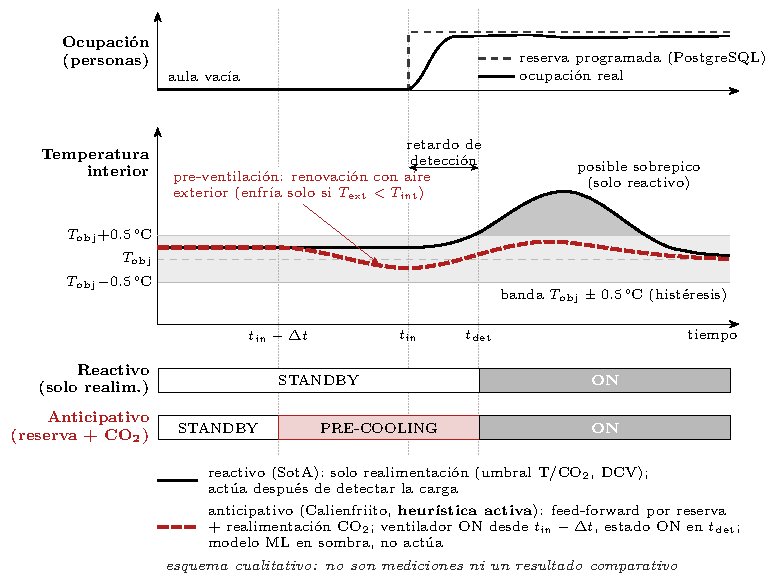
\includegraphics{figuras/diagramas/sota.pdf}
  \caption{Control reactivo frente a anticipativo ante el ingreso de ocupantes (esquema cualitativo; no representa mediciones). Fila superior: solo realimentación por umbral de temperatura o \COdos{}, como en la ventilación por demanda revisada~\cite{lu2022dcv,franco2020co2}. Fila inferior: acción \textit{feed-forward} a partir de la reserva del aula, corregida con el \COdos{} medido, en la línea de los controladores predictivos~\cite{gao2023comparative,kumkam2025comparative}. En Calienfriito esta lógica la ejecuta la heurística activa; el modelo ML corre en sombra con las mismas entradas.}
  \Description{Esquema cualitativo con dos filas: control reactivo que actúa tras detectar la carga y control anticipativo que ventila desde la reserva del aula; ocupación, temperatura y estados de decisión en función del tiempo.}
  \label{fig:sota}
\end{figure}

Las limitaciones de la Tabla~\ref{tab:sota} fijan el resto del diseño. En actuación y sensado, los nodos de monitoreo revisados no actúan~\cite{fayos2021ventqsys,mumtaz2021iot}, así que el nuestro comanda un ventilador por PWM, y el lazo cerrado de Sung y Hsiao~\cite{sung2020thermal}, limitado al confort térmico, lo ampliamos con el \COdos{} y la reserva del aula. La rama de potencia va separada de la lógica, la práctica con la que SmartFan eliminó sus reinicios~\cite{niamah2026esp32}, y el ventilador se conmuta con un MOSFET de nivel lógico en lugar de un puente bipolar. La calibración del MQ-135 de Dewi~\cite{dewi2025mq135} vale en laboratorio: tratamos su salida como índice relativo, la calibramos en dos puntos en el aula real y la contrastamos con el conteo de personas por cámara. La carcasa separa la cámara de sensado del flujo del ventilador, para no reproducir el sesgo de ubicación del sensor que documenta Lu~\cite{lu2022dcv}. El estudio de Cen~\cite{cen2024students} respalda el ventilador como actuador y motiva regular su velocidad con la temperatura medida.

En el modelo y los datos, la ocupación medida por \COdos{} se combina con la esperada según la reserva, porque el \COdos{} informa con retardo~\cite{franco2020co2,kallio2021forecasting}. De Kallio~\cite{kallio2021forecasting} tomamos dos prácticas: comparar siempre contra líneas base triviales y preferir modelos de árboles livianos. Mumtaz no contrasta su modelo con una regla~\cite{mumtaz2021iot}; nosotros fijamos las líneas base desde el diseño. La única comparación directa contra reglas que revisamos da una mejora de 3.29~\%~\cite{kumkam2025comparative}, y Gao y Wang superan a un PI tras 23 a 47 episodios simulados~\cite{gao2023comparative}, una exploración que en un aula real ocurriría durante clases. Por eso descartamos el aprendizaje por refuerzo, usamos regresión supervisada y dejamos el modelo en sombra. Nuestra hipótesis de trabajo es que una heurística bien calibrada puede bastar.

\subsection{Componentes y especificaciones}
La Tabla~\ref{tab:componentes} reúne los componentes del nodo con las especificaciones que determinan su integración. Los tres sensores ambientales son vitales para el lazo de control. El INA219 es adicional: sin él el sistema funciona igual, pero la potencia se reporta como estimación. La cámara con MediaPipe corre en un equipo externo y sirve para validar la ocupación estimada por \COdos{}.

\begin{table}[htbp]
\caption{Componentes del nodo y especificaciones clave según sus hojas de datos.}
\label{tab:componentes}
\footnotesize
\begin{tabularx}{\linewidth}{@{}P{2.2cm} Y Y P{1.7cm} P{2.1cm} Y@{}}
\toprule
Componente & Rango & Precisión / resolución & Tensión & Interfaz ESP32 & Consumo \\
\midrule
ESP32 (DevKit)~\cite{espressif2026esp32} & --- & ADC 12~bit & 3.3~V (VIN 5~V) & --- & TX 240~mA pico; RX 95--100~mA \\
DHT11~\cite{aosong2013dht11} & 0--50~\gradC{}; 20--90~\%HR & $\pm 2$~\gradC{}; $\pm 5$~\%HR; resolución 1~\gradC{} y 1~\%HR & 3.3~V propuesto (admite 3.3--5.5~V) & GPIO digital, bus de un hilo & 0.3~mA midiendo \\
MQ-135~\cite{hanwei2008mq135} & 10--1000~ppm según el gas & Índice relativo; $R_s/R_0$ & Calefactor 5~V & ADC1 vía divisor & $\leq 800$~mW (calefactor) \\
MQ-7~\cite{hanwei2007mq7} & 20--2000~ppm CO & Calibrado con $R_0$ en aire limpio & Calefactor 5~V / 1.4~V cíclico (propuesto) & ADC1 vía divisor; calefactor por MOSFET & $\approx 350$~mW promedio del ciclo (0.76~W en la fase de 5~V) \\
INA219~\cite{ti2015ina219} & Bus 0--26~V & $\leq 0.5$~\% (grado B) & 3.3~V (admite 3--5.5~V) & \IIC{} (0x40); shunt en la rama del ventilador (provisional) & $\leq 1$~mA \\
Ventilador DC & 0--100~\% PWM & --- & 12~V & LEDC $\to$ MOSFET lado bajo + diodo & \pendiente{corriente nominal del modelo (P-09)} \\
Buzzer + LED RGB & --- & --- & 3.3~V & GPIO digital & Solo en alarma \\
Calefactor PTC (opcional) & --- & --- & 12~V & GPIO $\to$ MOSFET o relé & \pendiente{potencia; confirmar si se monta (P-01)} \\
\bottomrule
\end{tabularx}
\end{table}

\subsection{Selección del microcontrolador}
Elegimos el ESP32 frente al ESP8266, al Arduino UNO R3 y a la Raspberry Pi Pico W; la Tabla~\ref{tab:mcu} resume la comparación.

\begin{table}[htbp]
\caption{Comparación de microcontroladores candidatos según sus hojas de datos.}
\label{tab:mcu}
\footnotesize
\begin{tabularx}{\linewidth}{@{}P{2.3cm} Y Y Y Y@{}}
\toprule
Característica & ESP32~\cite{espressif2026esp32} & ESP8266EX~\cite{espressif2025esp8266} & UNO R3 (ATmega328P)~\cite{microchip2018atmega328p} & Pico W (RP2040)~\cite{raspberrypi2026picow} \\
\midrule
CPU & 1 o 2$\times$ Xtensa LX6 según variante, hasta 240~MHz & 1$\times$ L106, hasta 160~MHz & AVR 8~bit, 16~MHz en la placa UNO R3 & 2$\times$ Cortex-M0+, 133~MHz \\
SRAM & 520~KB & $\approx 50$~KB disponibles & 2~KB & 264~KB \\
Flash & Externa (módulo) & Externa & 32~KB & 2~MB \\
ADC & 2$\times$12~bit, 18 canales (ADC1: 8 con WiFi); calibración en eFuse & 1$\times$10~bit, 0--1~V & 10~bit, 6 canales (PDIP) & 12~bit, 3 GPIO; errata de no linealidad (8.7 bits efectivos)~\cite{raspberrypi2025rp2040} \\
\IIC{} & 2 (hardware) & 1 (software) & 1 (TWI) & 2 \\
PWM & LEDC, 16 canales & 4 salidas & 6 canales & 16 canales \\
WiFi & Integrado & Integrado & No & Integrado (CYW43439) \\
\bottomrule
\end{tabularx}
\end{table}

El primer requisito es disponer de canales del convertidor analógico-digital (ADC) utilizables con WiFi activo. El nodo necesita dos entradas analógicas simultáneas (MQ-135 y MQ-7) mientras mantiene la conexión. El ESP32 integra dos convertidores de aproximaciones sucesivas (SAR) de 12~bit con 18 canales~\cite{espressif2026esp32}, pero el controlador WiFi usa el ADC2~\cite{espressif2026adc}, así que conectamos ambos sensores al ADC1, que ofrece 8 canales en los pines de entrada/salida de propósito general (GPIO) 32 a 39. El ESP8266 tiene un único ADC de 10~bit con entrada de 0 a 1.0~V~\cite{espressif2025esp8266}, insuficiente para dos sensores sin multiplexor externo.

La Pico W cumple en número de canales: expone tres GPIO con ADC~\cite{raspberrypi2026picow}. La diferencia está en la exactitud del convertidor. Su microcontrolador RP2040 tiene una errata del ADC sin corrección ni solución alternativa publicada: la no linealidad diferencial supera 1~LSB en los códigos 512, 1536, 2560 y 3584, y el número efectivo de bits medido baja a 8.7~\cite{raspberrypi2025rp2040}. El canal de seguridad de CO depende de ese convertidor. El ESP32 tampoco es ideal, porque su tensión de referencia varía entre 1000 y 1200~mV de un chip a otro, pero el fabricante graba parámetros de calibración en eFuse (en los chips que no los traen, el controlador usa una referencia por defecto) y ofrece un controlador de calibración que los aplica~\cite{espressif2026adccal}. Usamos esa calibración y, sobre ella, la calibración en dos puntos de cada sensor MQ.

El INA219 usa el bus \IIC{} (\textit{Inter-Integrated Circuit}) y el ventilador, PWM; ambos requieren periféricos por hardware. El ESP32 tiene dos controladores \IIC{} y un controlador PWM (LEDC, \textit{LED Control}) con 16 canales independientes, asignables a cualquier GPIO mediante la matriz de entrada/salida (E/S)~\cite{espressif2026esp32}. El ESP8266 implementa \IIC{} por software~\cite{espressif2025esp8266}.

En memoria y cómputo, el firmware mantiene simultáneamente la pila TCP/IP, el cliente MQTT con reconexión, la lectura de sensores y la lógica local de CO. El ESP32 dispone de 520~KB de SRAM y de uno o dos núcleos Xtensa LX6 de hasta 240~MHz según la variante del chip~\cite{espressif2026esp32}; el ESP8266 deja alrededor de 50~KB para \textit{heap} y datos~\cite{espressif2025esp8266}, y el ATmega328P del UNO tiene 2~KB de SRAM y 32~KB de Flash~\cite{microchip2018atmega328p}, sin radio. Si el módulo del DevKit es de doble núcleo, como los de la serie WROOM-32, podemos aislar la evaluación de CO de la gestión de red \pendiente{confirmar módulo del DevKit (p.\,ej. ESP32-WROOM-32E), número de núcleos y tamaño de Flash (P-10)}.

En conectividad, el ESP32 integra WiFi 802.11~b/g/n; el UNO requeriría un módulo externo. El ESP8266 figura como ``no recomendado para nuevos diseños'' en su hoja de datos vigente~\cite{espressif2025esp8266}. El costo energético de la radio es conocido: 240~mA en transmisión 802.11b a 19.5~dBm y 95--100~mA en recepción~\cite{espressif2026esp32}, valores que usamos en el presupuesto de potencia.

La Tabla~\ref{tab:gpio} propone la asignación de pines. Sigue cuatro criterios tomados de la hoja de datos~\cite{espressif2026esp32}. Los sensores MQ van al ADC1, y en él a GPIO34 y GPIO35, que son solo de entrada; así quedan libres los pines bidireccionales para las salidas. Evitamos los pines de arranque (\textit{strapping}) GPIO0, 2, 5, 12 y 15, cuyo nivel en el reinicio fija el modo de arranque, y los GPIO6 a 11, conectados a la memoria Flash. El bus \IIC{} usa GPIO21 y 22, asignados por la matriz de E/S, y cada salida PWM usa un canal LEDC propio. Si el módulo del DevKit integra PSRAM, GPIO16 y 17 quedan reservados para ella y el LED se reubica \pendiente{tabla de asignación de GPIO definitiva del firmware (P-06)}.

\begin{table}[htbp]
\caption{Asignación de GPIO propuesta para el ESP32 (propuesta de diseño; la definitiva depende del firmware, P-06).}
\label{tab:gpio}
\footnotesize
\begin{tabularx}{\linewidth}{@{}P{3.4cm} P{2.4cm} Y@{}}
\toprule
Señal & GPIO & Función del pin y motivo \\
\midrule
MQ-135, salida analógica & GPIO34 & ADC1\_CH6, solo entrada; vía divisor resistivo \\
MQ-7, salida analógica & GPIO35 & ADC1\_CH7, solo entrada; vía divisor resistivo \\
DHT11, datos & GPIO4 & Bidireccional, sin función de arranque; \textit{pull-up} a 3.3~V \\
INA219, SDA / SCL & GPIO21 / GPIO22 & Asignados al \IIC{} por la matriz de E/S, sin función de arranque; dirección 0x40 \\
Ventilador, PWM & GPIO25 & LEDC canal 0 $\to$ compuerta del MOSFET de lado bajo \\
Calefactor MQ-7 & GPIO26 & LEDC canal 1 $\to$ MOSFET del calefactor (ciclo 5/1.4~V) \\
Calefactor PTC (opcional) & GPIO27 & Salida digital $\to$ MOSFET o relé \\
Buzzer & GPIO18 & Salida digital \\
LED RGB (R, G, B) & GPIO16, 17, 19 & Salidas digitales; GPIO16 y 17 se cambian si el módulo tiene PSRAM \\
\bottomrule
\end{tabularx}
\end{table}

\subsection{Alimentación y presupuesto de potencia}
\label{sec:potencia}
La alimentación se organiza en tres rieles con tierra común (Figura~\ref{fig:bloques-hw}). Una fuente de 12~V~DC alimenta directamente la rama de potencia: el ventilador y, si se monta, el calefactor PTC. Un convertidor reductor (\textit{buck}) de 12~V a 5~V alimenta los calefactores de los sensores MQ y la entrada VIN del ESP32. El regulador lineal de la placa DevKit baja 5~V a 3.3~V para la lógica del ESP32 y el INA219. El ventilador se conmuta con un MOSFET de nivel lógico en el lado bajo, con diodo de rueda libre; la separación de rieles y el diodo evitan que los picos de corriente del motor lleguen al riel de 3.3~V.

\begin{figure}[htbp]
  \centering
  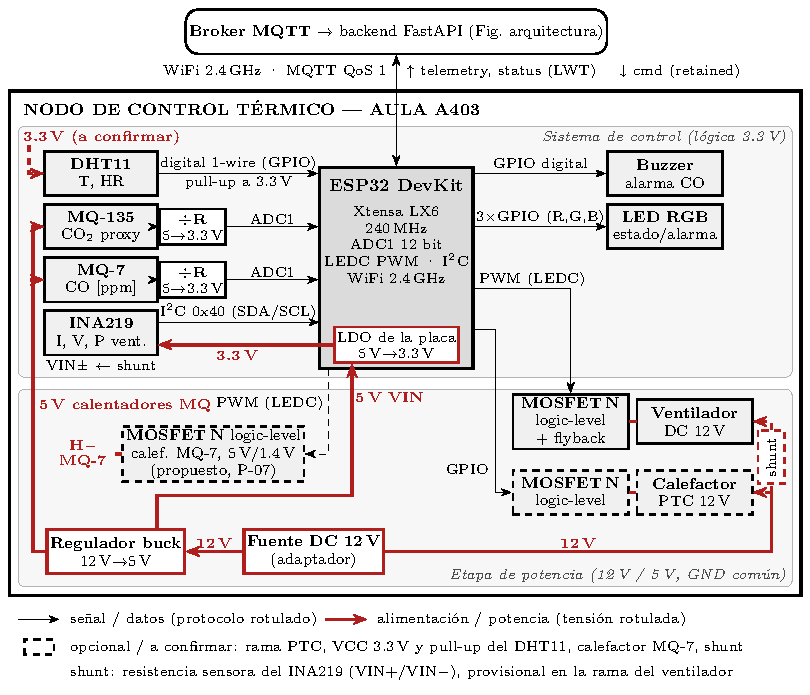
\includegraphics{figuras/diagramas/bloques-hw.pdf}
  \caption{Diagrama de bloques del hardware: rieles de 12~V, 5~V y 3.3~V, separación entre la rama de potencia y la de control, e interfaz de cada enlace (ADC1, \IIC{}, bus de un hilo, PWM LEDC, GPIO y WiFi).}
  \Description{Diagrama de bloques del hardware con rieles de alimentación de 12, 5 y 3.3 V, sensores, actuadores y protocolos de cada enlace.}
  \label{fig:bloques-hw}
\end{figure}

Proponemos alimentar el DHT11 desde el riel de 3.3~V, dentro de su rango de 3.3 a 5.5~V~\cite{aosong2013dht11}, con su resistencia de \textit{pull-up} conectada también a 3.3~V. Si el sensor y su \textit{pull-up} fueran a 5~V, la línea de datos llevaría 5~V a un GPIO del ESP32, cuya tensión de entrada no debe superar la de alimentación en más de 0.3~V~\cite{espressif2026esp32} \pendiente{confirmar tensión de alimentación y \textit{pull-up} del DHT11 montados (P-07)}.

El calefactor del MQ-7 requiere el ciclo de 5~V y 1.4~V descrito en la Sección~\ref{sec:marco}, que un riel fijo de 5~V no produce. Como diseño propuesto, un MOSFET de nivel lógico conmuta el calefactor desde el riel de 5~V, gobernado por un canal LEDC: 60~s a ciclo completo y 90~s a ciclo reducido. La potencia del calefactor depende del valor eficaz de la tensión, no del medio; para disipar lo mismo que con 1.4~V continuos, el ciclo de trabajo debe ser $D = (1.4/5)^2 \approx 0.08$, y no $1.4/5 = 0.28$, que solo iguala la tensión media. El firmware toma la lectura válida de CO al final de cada fase de 1.4~V \pendiente{confirmar si el calefactor del MQ-7 se cicla o queda fijo a 5~V (P-07)}. Si el equipo opta por dejarlo fijo a 5~V, como en muchos módulos comerciales, la salida se aparta de la hoja de datos y pasa a ser un índice con más sensibilidad cruzada, aunque la alarma podría evaluarse en cada lectura.

Las salidas analógicas de los módulos MQ llegan hasta 5~V, mientras que el ADC del ESP32 pierde exactitud por encima de unos 2450~mV con la atenuación máxima~\cite{espressif2026esp32}. Cada salida pasa, entonces, por un divisor resistivo con relación $R_2/(R_1+R_2) \leq 2.45/5 \approx 0.49$ \pendiente{valores de $R_1$ y $R_2$ montados (P-11)}.

El INA219 mide, de forma provisional, la rama del ventilador: su resistencia \textit{shunt} va en serie con el motor, en el lado de 12~V; así reporta la potencia del actuador y no la de la electrónica \pendiente{confirmar ubicación del \textit{shunt} del INA219 (P-06)}. En consecuencia, el consumo del nodo que muestra el dashboard es la suma de esa potencia medida y del valor nominal de la electrónica de la Tabla~\ref{tab:potencia}, y se etiqueta como estimado mientras la segunda parte no se mida.

La Tabla~\ref{tab:potencia} estima la potencia a partir de las hojas de datos. El riel de 5~V consume del orden de 1.65~W en operación continua, dominado por los calefactores de los sensores MQ. Para el MQ-7 promediamos el ciclo con la resistencia de calefactor de 33~$\Omega$ de su hoja de datos~\cite{hanwei2007mq7}: $(5^2/33 \times 60 + 1.4^2/33 \times 90)/150 \approx 0.34$~W. Si $\eta$ es la eficiencia del convertidor reductor, la electrónica demanda $1.65/\eta$~W de la fuente de 12~V. Para el ventilador el backend usa un valor nominal de 2.4~W (0.2~A a 12~V) hasta disponer de la medición del INA219.

\begin{table}[htbp]
\caption{Presupuesto de potencia estimado a partir de hojas de datos (no son mediciones).}
\label{tab:potencia}
\footnotesize
\begin{tabularx}{\linewidth}{@{}P{3.6cm} P{1.2cm} Y r@{}}
\toprule
Carga & Riel & Supuesto & Potencia [W] \\
\midrule
ESP32 con WiFi conectado & 5~V & 100~mA medios (RX 95--100~mA; picos TX de 240~mA) & 0.50 \\
Calefactor MQ-135 & 5~V & Máximo de hoja de datos & 0.80 \\
Calefactor MQ-7 & 5~V & Promedio del ciclo 60~s a 5~V y 90~s a 1.4~V sobre 33~$\Omega$ & 0.34 \\
DHT11 + INA219 & 3.3~V & 0.3~mA y 1~mA & $<0.01$ \\
\midrule
Subtotal electrónica & 5~V & & 1.65 \\
Electrónica vista desde 12~V & 12~V & $1.65/\eta$ & \pendiente{$\eta$ del buck (P-12)} \\
Ventilador al 100~\% & 12~V & Nominal del backend, 0.2~A & 2.4 \\
Calefactor PTC (opcional) & 12~V & & \pendiente{modelo (P-01)} \\
\bottomrule
\end{tabularx}
\end{table}

Con estos supuestos, la electrónica consume $1.65~\mathrm{W}\times 24~\mathrm{h} \approx 40$~Wh por día en el riel de 5~V, y el ventilador a plena velocidad durante 8~h de clases añade 19.2~Wh. Con $\eta = 0.85$ el total estimado es de unos 66~Wh diarios sin calefactor, unos 2~kWh al mes y 24~kWh al año. Como precio de referencia tomamos el cargo por energía de la tarifa BT5B no residencial de Luz del Sur, la distribuidora de Barranco, vigente desde el 4 de agosto de 2026: S/~0.7556 por kWh con el impuesto general a las ventas (IGV)~\cite{luzdelsur2026pliego}. Con ese precio, el costo estimado del nodo es de unos S/~0.05 por día, S/~1.5 al mes y S/~18 al año por aula. Es una referencia, no la factura real: el campus puede pagar otra opción tarifaria, por ejemplo en media tensión \pendiente{opción tarifaria y precio por kWh que paga UTEC Barranco (P-01)}. El promedio de 1.65~W sirve para la energía y el costo, pero la fuente se dimensiona para el peor caso simultáneo: el ESP32 transmitiendo (240~mA a 5~V, 1.2~W), el calefactor del MQ-135 (0.80~W) y el del MQ-7 en su fase de 5~V ($5^2/33 \approx 0.76$~W) suman 2.76~W en el riel de 5~V, a los que se añade el ventilador al 100~\%. Con un margen del 25~\%, la corriente de la fuente debe cumplir $I \geq 1.25\,(2.76/\eta + 2.4 + P_{\mathrm{PTC}})/(12~\mathrm{V})$. Si se toma $\eta = 0.85$, valor típico de un convertidor reductor que debe confirmarse con el modelo instalado, el requisito sin calefactor es de unos 0.6~A \pendiente{corriente nominal de la fuente instalada (P-01)}.

\subsection{Arquitectura de comunicación y software}
\label{sec:comunicacion}
La Figura~\ref{fig:arquitectura} muestra las capas del sistema. En el diseño del nodo, la telemetría y el comando viajan por MQTT. El nodo publica en \texttt{ccs/<room>/telemetry} con QoS~1: temperatura, humedad, \COdos{} relativo, CO, potencia, corriente, tensión de bus, ciclo PWM, estado del calefactor y de la alarma, indicador de intensidad de señal recibida (RSSI) y tiempo desde el arranque del nodo (\texttt{uptime\_s}). Al conectarse, publica \texttt{online} (retenido) en \texttt{ccs/<room>/status} y registra \texttt{offline} en el mismo tópico como última voluntad. En el backend FastAPI, el puente MQTT está desactivado por defecto y se activa al configurar la dirección del broker. Activo, se suscribe a \texttt{ccs/+/telemetry} y \texttt{ccs/+/status}, valida cada lectura, la guarda en MongoDB junto con la decisión y publica el comando en \texttt{ccs/<room>/cmd} con QoS~1 y la bandera RETAIN, para que un nodo que se reinicia reciba el último comando al suscribirse. El comando contiene la acción, el PWM base, el estado del calefactor (campo reservado: el backend aún no lo asigna, P-01), el motivo, el controlador activo y la consigna ajustada $T^{*}$ (campo \texttt{target}).

\begin{figure}[htbp]
  \centering
  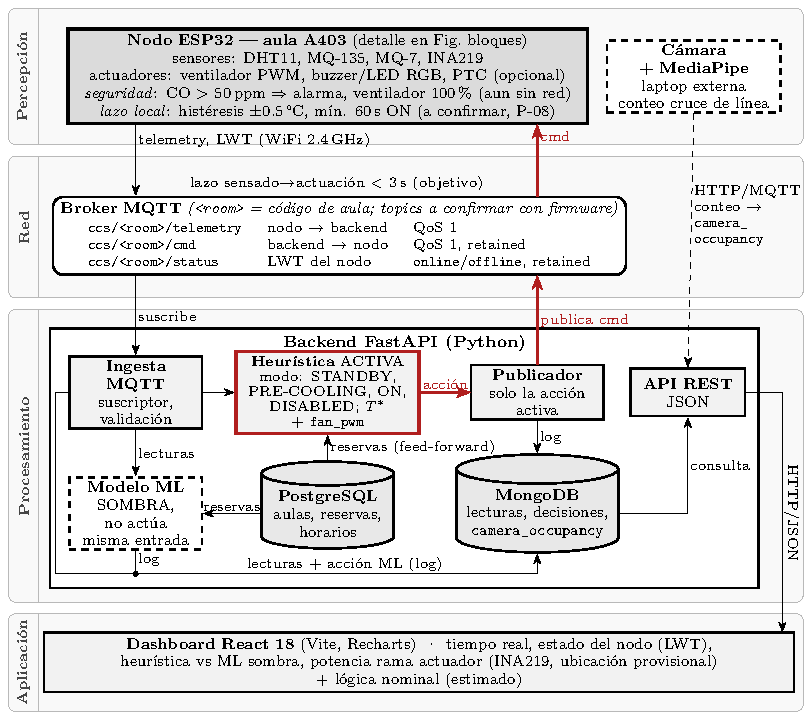
\includegraphics{figuras/diagramas/arquitectura.pdf}
  \caption{Arquitectura del sistema: nodo ESP32, broker MQTT con tópicos de telemetría, comando retenido y estado (LWT), backend FastAPI con MongoDB y PostgreSQL, y dashboard React.}
  \Description{Arquitectura en capas: nodo ESP32, broker MQTT, backend con bases de datos y dashboard web.}
  \label{fig:arquitectura}
\end{figure}

\textit{Medición de la latencia.} Para que la latencia sensado$\to$actuación sea medible, el contrato del comando incorpora el campo \texttt{src\_ts}: la marca de tiempo de la lectura que originó la decisión, copiada sin cambios de la telemetría. La respuesta HTTP de la decisión devuelve el mismo campo. Por diseño, el nodo sincroniza su reloj por SNTP (protocolo simple de tiempo de red) al conectarse y sella cada lectura con esa hora. Al recibir el \texttt{cmd} y escribir el registro LEDC, calculará la latencia como su hora local menos \texttt{src\_ts} y la reportará en el campo \texttt{latency\_ms} de la telemetría siguiente. Contamos como actuación la aplicación del comando, aunque el lazo local difiera el cambio de estado del ventilador por la banda o el encendido mínimo. Las dos marcas salen del mismo reloj del nodo, de modo que el desfase entre el nodo y el servidor no entra en la medida. El error que queda es la deriva del reloj durante unos pocos segundos y cualquier corrección SNTP aplicada entre la lectura y la recepción; el firmware debe marcar y descartar esas muestras. Un \texttt{cmd} cuyo \texttt{src\_ts} no corresponde a una lectura del nodo, como uno retenido de una sesión anterior, no produce muestra de latencia \pendiente{implementar \texttt{src\_ts} en el backend y la medición en el firmware (P-20)}.

El backend acepta también lecturas por HTTP (\texttt{POST /api/v1/sensors/}). Es la vía de las aulas simuladas y la de respaldo durante el desarrollo. Cada lectura se procesa y se guarda igual, y la respuesta HTTP devuelve la decisión al cliente que envió la lectura; esta vía no publica comando retenido ni ofrece última voluntad. Un nodo que la use recibe la decisión en la respuesta a su propia petición, opera con su lazo local entre peticiones y no recupera el comando tras reiniciarse. Mientras el piloto no se ejecute, no afirmamos que la ruta MQTT opere en producción.

PostgreSQL guarda aulas, horarios y reservas, de donde sale la ocupación esperada. El dashboard React consulta indicadores ya procesados por el backend: latencia p95, disponibilidad del nodo, cumplimiento del encendido mínimo, alarmas de CO resueltas localmente frente a las del servidor y energía y costo del propio nodo. La potencia del nodo que muestra es la de la rama del ventilador medida por el INA219 más la de la electrónica según su valor nominal, rotulada como estimada; cada lectura declara además su procedencia (campo \texttt{data\_origin}), y el dashboard marca como ``origen no declarado'' las que no la traen. \pendiente{confirmar nombres de tópicos y campos con el firmware final (P-01)}

\subsection{Lógicas de decisión}
\label{sec:decision}
Ambas lógicas se ejecutan en el backend sobre cada lectura y emiten una de tres acciones: \texttt{ON}, \texttt{PRE-COOLING} o \texttt{STANDBY}. Cuando el control del aula está deshabilitado, el backend publica \texttt{DISABLED} sin ejecutarlas, y ese comando no lleva PWM ni consigna. Conservamos el nombre \texttt{PRE-COOLING} de la primera entrega, aunque un ventilador no enfría el aire: en Calienfriito equivale a ventilación anticipada antes de la clase. Las dos lógicas comparten la regla de decisión y difieren en cómo estiman la carga térmica $L$ del aula.

\textit{Ocupación efectiva.} La ocupación esperada $N_e$ sale de la reserva del aula y se considera activa desde 30~min antes del inicio de la clase. La ocupación medida $\hat N$ sale del \COdos{} (Sección~\ref{sec:marco}). El backend combina ambas como $N_{\mathrm{ef}} = 0.4\,N_e + 0.6\,\hat N$; si no hay lectura de \COdos{}, usa $N_e$.

\textit{Heurística (activa).} Estima $L = 0.05~\text{\gradC{}} \times N_{\mathrm{ef}}$ y calcula la consigna ajustada $T^{*} = T_{\mathrm{obj}} - L$. Si $T > T^{*}$, la acción es \texttt{ON}, o \texttt{PRE-COOLING} cuando hay una reserva próxima y el \COdos{} indica aula vacía ($\hat N < 1$); el ventilador recibe $\mathrm{PWM} = \min(100, \max(40, 40 + 40\,(T-T^{*})))$~\%. En otro caso la acción es \texttt{STANDBY}. Los pesos 0.4 y 0.6, los 30~min de anticipación, los 0.05~\gradC{} por persona y la ganancia de 40~\% por \gradC{} son valores iniciales que elegimos y que el experimento E4 recalibra con los datos reales. El piso de 40~\% evita comandar al ventilador por debajo de su ciclo mínimo de arranque \pendiente{medir el PWM mínimo de arranque del ventilador instalado (P-17)}. Si se monta el PTC, el diseño prevé un estado adicional, \texttt{HEATING}, que lo encendería cuando $T < T^{*} - h$; el backend actual no lo emite \pendiente{decidir si se monta el PTC y se implementa \texttt{HEATING} (P-01)}.

\textit{Lazo local en el nodo.} La heurística del servidor no aplica banda: compara $T$ con $T^{*}$ en cada lectura y publica modo y PWM. Por diseño, la histéresis de $\pm 0.5$~\gradC{} y el encendido mínimo de 60~s se asignan al lazo local del firmware (Figura~\ref{fig:flujo}): el nodo empieza a ventilar si $T > T^{*} + h$, con un PWM nunca menor que el piso de 40~\%, y deja de hacerlo si $T < T^{*} - h$ y el ventilador lleva al menos 60~s encendido. El mínimo es de encendido: retrasa el paso de encendido a apagado, pero no el de apagado a encendido. Un comando \texttt{DISABLED} apaga el ventilador sin esperar ese mínimo. El nodo obtiene $T^{*}$ del campo \texttt{target} del comando. \pendiente{confirmar implementación de histéresis y encendido mínimo en el firmware (P-08)}

\textit{Anticipación y banda local.} La anticipación no proviene de una excepción en el lazo local sino de la consigna. Con una reserva próxima, $N_{\mathrm{ef}}$ crece antes de que lleguen los estudiantes, $T^{*}$ baja y la banda de $\pm h$ actúa alrededor de esa consigna ya reducida. En \texttt{PRE-COOLING} el aula está vacía, así que $N_{\mathrm{ef}} \approx 0.4\,N_e$ y $L \approx 0.02\,N_e$: con $N_e = 40$, $L = 0.8$~\gradC{} y el nodo ventila si $T > T_{\mathrm{obj}} - 0.3$~\gradC{}. Este diseño tiene una limitación que declaramos. El backend emite \texttt{PRE-COOLING} cuando $T > T^{*}$, pero el nodo enciende el ventilador recién con $T > T^{*} + h$; si $T^{*} < T \leq T^{*} + h$ y el ventilador estaba apagado, no hay ventilación anticipada. Con reservas de menos de 25 personas ($L < h$), el umbral de encendido $T_{\mathrm{obj}} - L + h$ queda por encima de $T_{\mathrm{obj}}$, y la anticipación ocurre únicamente si el aula ya supera la consigna nominal.

\textit{Registro de ciclos del ventilador.} Para verificar el encendido mínimo sin depender del periodo de publicación, el contrato de telemetría del firmware incluye dos campos opcionales que el nodo llenará en el mensaje siguiente a cada paso de encendido a apagado: \texttt{fan\_on\_s}, la duración del ciclo medida con el reloj del nodo, y \texttt{fan\_off\_cause}, que vale \texttt{local} si el ciclo lo cerró la histéresis, \texttt{disabled} si lo cerró un comando \texttt{DISABLED} y \texttt{co\_alarm} si durante el ciclo intervino una alarma de CO. OE4 se evalúa sobre los ciclos con causa \texttt{local} \pendiente{implementar \texttt{fan\_on\_s} y \texttt{fan\_off\_cause} en el firmware (P-08, P-20)}.

\textit{Modelo ML (sombra).} Un \texttt{HistGradientBoostingRegressor} estima $L$ a partir de la temperatura, la hora, la ocupación esperada y la medida, la temperatura exterior y metadatos físicos del aula (piso, volumen y capacidad de climatización). Con ese $L$ aplica la misma regla y produce su propia acción, que se registra junto a la de la heurística pero no se publica al nodo. La diferencia entre ambas no está en la regla sino en la información: el modelo usa variables, como la temperatura exterior y el volumen del aula, que la heurística ignora.

\textit{Estado actual del modelo.} Hoy la canalización entrena el modelo con un conjunto sintético de aulas de UTEC que generamos para probarla, y con una etiqueta también sintética: \texttt{target\_temp\_offset} se calcula con una fórmula a partir de la ocupación, la temperatura y factores del aula. Un modelo que aprende esa fórmula reproduce variables que la heurística no ve, así que compararlo con la heurística sobre esa etiqueta no sería justo. No usamos esas métricas para decidir nada ni las reportamos como resultados.

\textit{Evaluación con datos reales.} Con la telemetría del A403 reentrenaremos el modelo para predecir una variable observable, el cambio de temperatura a 15~min, $\Delta T_{15} = T(t+15~\mathrm{min}) - T(t)$. Entre sus entradas incluiremos el PWM medio aplicado al ventilador en la ventana $[t, t+15~\mathrm{min}]$. Así la etiqueta existe en todas las ventanas, con el ventilador encendido o apagado, y no únicamente en las de baja carga, y el modelo puede separar el efecto del ventilador de la carga del aula. Lo comparamos con dos líneas base simples: la persistencia, que predice $\Delta T_{15} = 0$, y la media de $\Delta T_{15}$ en el conjunto de entrenamiento condicionada al estado del ventilador (apagado o encendido durante la mayor parte de la ventana). Calcularemos RMSE y MAE de las tres predicciones sobre un \textit{holdout} cronológico (último 20~\% de los datos, separado del entrenamiento por 15~min para que ninguna ventana cruce el corte) y ajustaremos los hiperparámetros con validación cruzada temporal de tres pliegues dentro del entrenamiento. Se descartan las ventanas con huecos de telemetría o con alarma de CO. El modelo supera a una línea base si el intervalo de confianza del 95~\% de la diferencia de RMSE (modelo menos línea base), estimado por \textit{bootstrap} de bloques diarios, queda por debajo de cero. La heurística no predice $\Delta T_{15}$: su $L$ es un desplazamiento de consigna, no un pronóstico, y por eso no entra en esta comparación; la concordancia de acciones entre heurística y modelo se reporta como dato descriptivo. Superar las líneas base es condición necesaria, no suficiente, para usar el modelo como controlador. Esa adopción queda como trabajo futuro y exigiría además una prueba A/B controlada en aula \pendiente{reentrenamiento del modelo con la etiqueta $\Delta T_{15}$ sobre datos reales del A403 (P-21)}.

\subsection{Carcasa}
Diseñamos una carcasa de dos piezas, base y tapa, para impresión en ácido poliláctico (PLA). La forma de la carcasa sigue tres requisitos: la rejilla de admisión y el ducto de descarga se alinean con el ventilador; la cámara de sensado queda ventilada y separada del flujo forzado, para que los MQ midan el aire del aula y no el que mueve el propio sistema; y el calor de los calefactores MQ se disipa lejos del DHT11. El diseño incluye postes M3, pasacables con alivio de tensión y una ventana para el LED de alarma. Si la impresión no estuviera lista, el plan alternativo es una caja reutilizada o de acrílico o de tablero de fibra de densidad media (MDF) con las mismas aberturas \pendiente{estado final de la carcasa y de la PCB propia (P-13)}.

%% =====================================================================
\FloatBarrier
\section{Implementación}
\label{sec:implementacion}

\subsection{Lógica del firmware}
La Figura~\ref{fig:flujo} describe el diseño del firmware del nodo \pendiente{enlace al repositorio o \textit{commit} del firmware (P-20)}. Al arrancar, el ESP32 inicializa los periféricos (ADC1, \IIC{}, LEDC y GPIO), se conecta a WiFi y al broker registrando el LWT, y se suscribe al tópico de comandos, del que recibe de inmediato el último comando retenido. Los sensores MQ requieren un periodo de precalentamiento antes de que sus lecturas sean válidas, y durante ese periodo la alarma de CO permanece inhibida. En cada ciclo el nodo lee los sensores y evalúa primero, en local, la última lectura válida de CO, que con el ciclo propuesto del calefactor llega al final de cada fase de 1.4~V: si supera 50~ppm, enciende buzzer y LED y lleva el ventilador al 100~\% sin esperar al servidor. Usamos 50~ppm como umbral instantáneo, un criterio conservador: el límite de OSHA es un promedio de 8~h y el techo de NIOSH es 200~ppm~\cite{osha2026co}. La alarma queda enclavada hasta que el CO baja de $50 - h_{\mathrm{CO}}$~ppm \pendiente{valor de la histéresis $h_{\mathrm{CO}}$ del umbral de CO (P-18)}. Sin alarma, aplica el último comando válido con la histéresis y el encendido mínimo de la Sección~\ref{sec:decision}, y después publica la telemetría del ciclo. Si pierde la conexión, mantiene la evaluación local de CO, apaga el PTC, lleva el ventilador a un estado seguro \pendiente{definir si el ventilador mantiene el último PWM o pasa a un valor fijo sin red (P-19)} y reintenta la conexión con espera creciente, sin bloquear el lazo \pendiente{duración del precalentamiento de los MQ, periodo de muestreo y de publicación, frecuencia LEDC y \textit{keepalive} configurados en el firmware (P-14)}.

\begin{figure}[htbp]
  \centering
  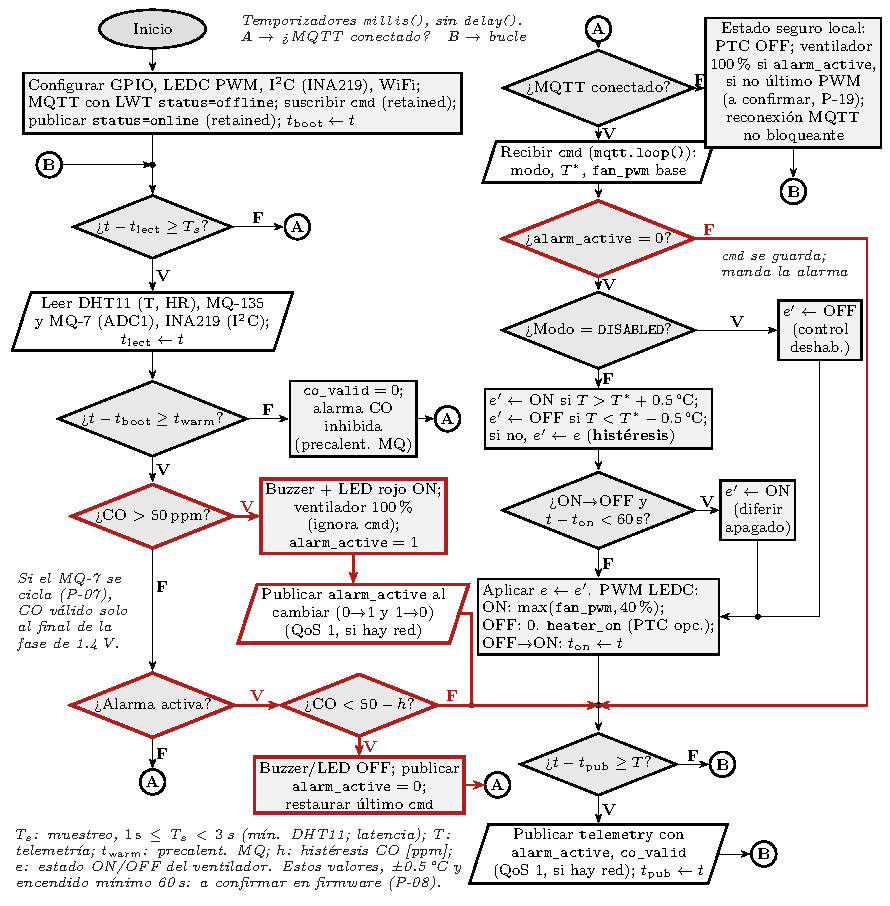
\includegraphics[width=0.9\linewidth]{figuras/diagramas/flujo.pdf}
  \caption{Diagrama de flujo del firmware: arranque, precalentamiento de sensores MQ, lazo de lectura, evaluación local de CO con prioridad, publicación MQTT, aplicación del comando con tiempo mínimo y modo seguro ante pérdida de conexión.}
  \Description{Diagrama de flujo del firmware del nodo, con la evaluación local de CO como rama prioritaria.}
  \label{fig:flujo}
\end{figure}

\subsection{Backend y dashboard}
El backend recibe cada lectura, estima la ocupación, ejecuta la heurística y el modelo en sombra, y guarda en MongoDB la lectura con ambas acciones, sus motivos y el controlador activo. Sobre esa colección calcula los indicadores de funcionamiento que muestra el dashboard: latencia sensado$\to$actuación (mediana y p95 frente al objetivo de 3~s), caídas del enlace detectadas como huecos mayores a tres veces el periodo nominal, cumplimiento del encendido mínimo, confort, alarmas de CO resueltas en el nodo frente a las detectadas solo en el servidor, y energía y costo del nodo por día, mes y año. El confort es el porcentaje de muestras con la temperatura dentro de $\pm 1$~\gradC{} del objetivo configurado del aula, no de $T^{*}$. La banda es asimétrica: las muestras por encima se atribuyen al control, y las que quedan por debajo se cuentan aparte como aula fría, fuera del alcance de un ventilador, sin penalizarlo. Cuando una lectura no trae potencia medida, el dashboard la etiqueta como ``estimada'' y usa los valores nominales de la Sección~\ref{sec:potencia}. La tarifa es configurable; por defecto el backend usa la de referencia de la Sección~\ref{sec:potencia}, S/~0.7556 por kWh, y la rotula como no confirmada mientras no se conozca la que paga el campus. Las pruebas automáticas del backend (\texttt{pytest}) cubren estos cálculos.

\subsection{Prototipo}
La Figura~\ref{fig:fotos} reúne las fotografías del prototipo. La Figura~\ref{fig:bloques-hw} es la referencia de interconexión para el montaje.

\begin{figure}[htbp]
  \centering
  \fbox{\parbox[c][2cm][c]{0.9\linewidth}{\centering\pendiente{fotos reales: (a) nodo armado en protoboard o PCB, (b) interior de la carcasa con la cámara de sensado separada, (c) nodo instalado en el aula A403 (P-02)}}}
  \caption{Prototipo de Calienfriito. \pendiente{pie definitivo que explique qué muestra cada foto (P-02)}}
  \Description{Espacio reservado para las fotografías del prototipo.}
  \label{fig:fotos}
\end{figure}

%% =====================================================================
\FloatBarrier
\section{Análisis de resultados}
\label{sec:resultados}
A la fecha de esta versión no contamos con telemetría del nodo físico en el aula A403, y esta sección no reporta resultados. Ningún número de este informe proviene de mediciones nuestras; los de la Sección~\ref{sec:potencia} son estimaciones de hoja de datos. \pendiente{resultados reales de los experimentos E1--E5 (P-03)}

La Tabla~\ref{tab:plan} define los experimentos que alimentan esta sección. Cada uno se asocia con un objetivo de la Tabla~\ref{tab:objetivos} y usa lecturas con \texttt{is\_simulated} igual a falso.

\begin{table}[htbp]
\caption{Plan experimental en el aula A403.}
\label{tab:plan}
\footnotesize
\begin{tabularx}{\linewidth}{@{}l Y Y P{2.2cm} l@{}}
\toprule
ID & Procedimiento & Métrica & Duración & Objetivo \\
\midrule
E1 & Operación continua del nodo en el aula con clases normales; conteo manual de personas para recalibrar $k$. & Lecturas válidas (\%), huecos de enlace, disponibilidad. & 7 días hábiles & OE1, OE2 \\
E2 & El nodo sella cada lectura con su reloj sincronizado por SNTP; al aplicar un \texttt{cmd} resta su \texttt{src\_ts} (Sección~\ref{sec:comunicacion}). & Latencia mediana y p95. & Dentro de E1 & OE2 \\
E3 & Broker apagado; umbral de CO reducido en una versión de prueba del firmware. & Tiempo desde la lectura válida de CO hasta alarma y PWM 100~\%. & 10 repeticiones & OE3 \\
E4 & Registro de decisiones heurística y ML en sombra; reentrenamiento del modelo con los datos de E1. & Ciclos con causa \texttt{local} y \texttt{fan\_on\_s} $\geq 60$~s; RMSE y MAE de $\Delta T_{15}$ del modelo frente a persistencia y media condicionada; concordancia de acciones (descriptiva). & Dentro de E1 & OE4, OE5 \\
E5 & Potencia del INA219, en modo de promedio de 128 muestras~\cite{ti2015ina219}, frente a multímetro con PWM de 0, 50 y 100~\%. & Error relativo (\%). & 3 puntos $\times$ 5 lecturas & OE6 \\
\bottomrule
\end{tabularx}
\end{table}

La Figura~\ref{fig:resultados-telemetria} se genera con el script \texttt{figuras/resultados/graficar\_resultados.py} a partir de la exportación de MongoDB del aula A403. El script descarta las lecturas simuladas y no escribe la figura si no hay datos reales; el documento la incluye automáticamente en cuanto el archivo existe.

\begin{figure}[htbp]
  \centering
  \IfFileExists{figuras/resultados/resultados-telemetria.pdf}{%
    \includegraphics[width=0.9\linewidth]{figuras/resultados/resultados-telemetria.pdf}%
  }{%
    \fbox{\parbox[c][3cm][c]{0.9\linewidth}{\centering\pendiente{figura original con datos reales del aula A403 (requiere exportación de telemetría; ver PENDIENTES P-03)}}}%
  }%
  \caption{Telemetría real del nodo en el aula A403: temperatura y consigna ajustada, \COdos{} relativo y CO, ciclo PWM y potencia medida, y acciones de la heurística activa frente al modelo en sombra.}
  \Description{Series de tiempo de temperatura, gases, PWM, potencia y acciones de decisión del nodo en el aula A403.}
  \label{fig:resultados-telemetria}
\end{figure}

%% =====================================================================
\FloatBarrier
\section{Descripción del mercado}
\label{sec:mercado}
El segmento inicial son las universidades privadas peruanas con edificios climatizados de forma centralizada y aulas de ocupación variable, el tipo de espacio donde la ventilación por demanda rinde más~\cite{lu2022dcv}. Tras el primer licenciamiento institucional, la oferta universitaria del país quedó en 92 universidades y dos escuelas de posgrado; de esas 94 instituciones licenciadas, 48 eran privadas, y entre todas sumaban 358 locales autorizados~\cite{sunedu2022bienal}. El cliente es el área de infraestructura del campus; el usuario final es el estudiante, que recibe aire renovado y alertas de CO, y el docente, que ve el estado del aula en el dashboard. Calienfriito no reemplaza al sistema central: se instala aula por aula, a baja tensión y sin intervenir la red eléctrica, y eso reduce la barrera de adopción \pendiente{costo de materiales del nodo en S/ (P-15)}.

El modelo de negocio combina la venta del nodo con una suscripción por aula que incluye el broker, el backend, el dashboard y el reentrenamiento periódico del modelo con los datos de cada campus. El costo de operación del nodo es el argumento central de venta: según el presupuesto estimado de la Sección~\ref{sec:potencia}, que la Figura~\ref{fig:mercado-consumo} desglosa por carga, el nodo consume del orden de 2~kWh al mes sin calefactor, un costo estimado de S/~1.5 al mes por aula a la tarifa de referencia de Luz del Sur~\cite{luzdelsur2026pliego}. Recalcularemos esa cifra con la potencia medida en E5 y la tarifa real del campus; el precio de venta del nodo se fijará sobre su costo de materiales \pendiente{precio objetivo del nodo a partir del costo de materiales (P-15)}. El video publicitario presenta el prototipo y este argumento: \pendiente{enlace al video publicitario: \url{URL-PENDIENTE} (P-04)}.

\begin{figure}[htbp]
  \centering
  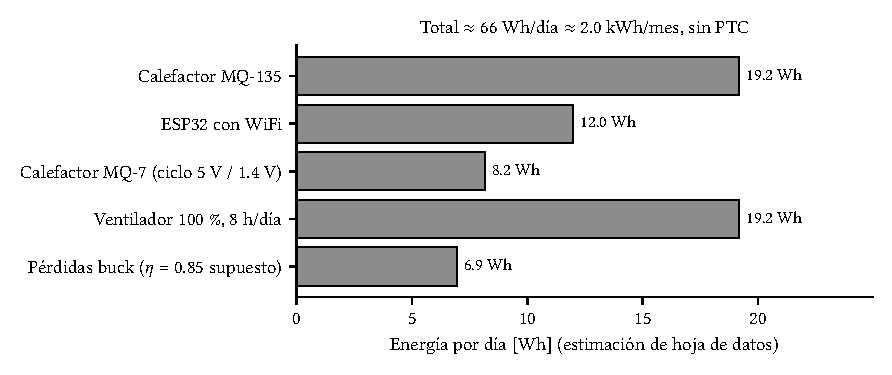
\includegraphics[width=\linewidth]{figuras/mercado/consumo-estimado.pdf}
  \caption{Energía diaria estimada del nodo por carga, a partir de la Tabla~\ref{tab:potencia} (hojas de datos; no son mediciones) con $\eta = 0.85$ supuesto para el convertidor reductor. Generada con \texttt{figuras/mercado/graficar\_consumo\_estimado.py}; se rehará con la potencia medida en E5.}
  \Description{Barras horizontales con la energía diaria estimada de cada carga del nodo: calefactores MQ, ESP32, ventilador y pérdidas del convertidor; total cercano a 66 Wh por día.}
  \label{fig:mercado-consumo}
\end{figure}

%% =====================================================================
\FloatBarrier
\section{Conclusiones y recomendaciones}
\label{sec:conclusiones}
Diseñamos un nodo IoT que cierra un lazo de sensado, decisión y actuación por aula con componentes de bajo costo y baja tensión. La elección del ESP32 responde a requisitos verificables: dos entradas analógicas en ADC1 utilizables con WiFi activo, \IIC{} y PWM por hardware, 520~KB de SRAM y radio integrada. La alimentación separa la rama de 12~V de la lógica, y su presupuesto, estimado a partir de hojas de datos, indica que los calefactores de los sensores MQ, y no el microcontrolador, dominan el consumo continuo del nodo.

La revisión del estado del arte mostró que los nodos de monitoreo no actúan, que el lazo cerrado revisado se limita al confort térmico y que los controladores aprendidos se validan en simulación, con ganancias pequeñas frente a reglas en el único estudio que las compara directamente. El aporte que persigue Calienfriito es evaluar en campo, sobre las mismas lecturas con que opera una heurística, si un modelo aprendido predice una variable observable ($\Delta T_{15}$) mejor que predictores triviales, y no sobre la etiqueta sintética con que hoy se entrena. Ese resultado es la primera condición para que el modelo justifique su complejidad; su uso como controlador requeriría además una prueba A/B en aula. \pendiente{conclusiones basadas en los resultados de E1--E5 (P-03)}

Como trabajo futuro, reemplazar el MQ-135 por un sensor NDIR de \COdos{} cuando el presupuesto lo permita llevaría la medición de un índice relativo a ppm absolutas. Operar el nodo durante un semestre completo antes de decidir sobre el modelo cubriría la variación estacional de Lima. Conviene también medir el calentamiento que los calefactores MQ inducen en el DHT11 dentro de la carcasa y, si se adopta, colocar el \textit{shunt} del INA219 en la entrada de 12~V para medir el nodo completo y no solo su actuador.

%% =====================================================================
\FloatBarrier
\bibliographystyle{IEEEtran}
\bibliography{referencias}

\end{document}
